%% It is just an empty TeX file.
%% Write your code here.
\chapter{Experiment}

The communication is essential for the proper functionality of most systems. Every smallest peace of electronics is somehow connected to others and with the IoT era it will only grow in popularity. With todays technologies many connections can be performed without the use of any physical medium, like wires or fiber-optics. The wireless technologies are commonly used not only in cellular networks but more and more commonly in the short range communication and even industrial applications. Very in particular interesting subject is the problem of communicating systems placed on robotic arms that tend to move and rotate leading to fast deterioration of cables and plugs.
The goal of the ParSec project is to create a dependable, flexible and secure wireless communication system which meets all industrial automation requirements. It has to work with latencies below 1 ms and with very high noise level, serving many distributed clients at once. Moreover it has to deal with fading effects and potentially many reflections or even obstacles coming in the way of transmission and breaking it. The part of the work, that has been assigned to the Faculty of Technical Informatics at the Brandenurg University of Technology Cottbus-Senftenberg was to cover the dependability of the wireless communication. 

\section{Communication Systems}
The communication and storage of the information was a subject of much research going back to the half of the last century. The models created back then are still valid and have been only extended. \autoref{fig:data_path} shows an abstraction of the transmission path, a very common communication model.
\begin{figure}[H]
\centering
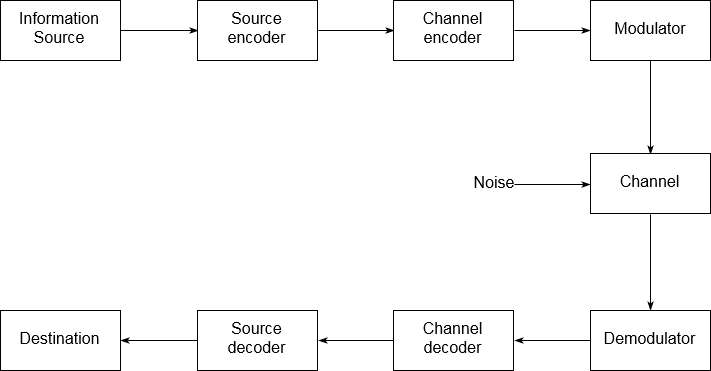
\includegraphics[width=0.65\textwidth]{figures/Data_transmission_path.png}
\caption{Block diagram of a typical data transmission (storage) system~\cite{book:LinCostello}}
\label{fig:data_path}
\end{figure}

The digital source of information can be understood as a MAC layer, followed by:
\begin{itemize}
    \item source encoder - compresses the data by removing useless redundancy, leaving just the information that needs to be transmitted. In other words, a perfectly designed source encoder minimizes the number of bits per unit time needed to represent the source information. Since every bit of compressed information is significant, than decoding a sequence with changed bits would produce catastrophic results.
    \item cryptography encoder - helps to protect the confidentiality and integrity of data being sent, meaning that it cannot be read or altered by unauthorized third parties. It adds useful redundancy to protect the information contained in the message. Cryptography by itself doesn't guarantee any security when not combined with other security means. Without secure key management protocols and thoughtful design the security can be easily compromised. More information can be found in~\cite{Cryptography}. In many cases, one of the encryption stages involves using hash functions which counteracts the manipulation of encrypted bitstream. The hashing algorithm produces a unique output for each individual input, making it impossible to alter the transmitted information without corrupting it. Channing one bit within hashed bitstream leads to decryption of a completely different clear text.
    \item channel encoder - transforms the \textit{information sequence} \textbf{u}, produced by digital source (MAC layer, source encoder or cryptography encoder), into a \textit{code~word} \textbf{v}. It adds useful information redundancy, which allows the channel decoder to detect transmission errors. The simplest example is a parity bit added at the end of a message indicating an odd or even number of ones in the message. More complicated approaches, together with Forward Error Correction were described in \autoref{sec:coding}.
    \item modulator - since the discrete symbols are not applicable for transmission they need to be translated into the waveform and then sent to the receiver, that's why the channel encoder is followed by the modulator~\cite{book:LinCostello}. The sending of the waveform takes part in the Radio Frequnecy module. Modulators, together with frame formatters, DC/AC converters, symbol shaping modules and RF modules are nowadays parts of the baseband processors~\cite{book:Ismail}. The baseband processors are mixtures of digital and analog components.
\end{itemize}
\section{FEC in Communication Systems}
Various signals transmitted in industrial environment have different requirements in terms of dependability. Let's consider a simple CCTV video transmission system. Each frame, even in low resolution solutions, consists of several hundred thousands pixels. The frame rate lies somewhere between 30 and 5 frames per second, depending on the requirements. Even multiple bit error in the compressed video information bitstream leads just to the corruption of some frames. Depending on the error rate and frame rate, such disturbance may not influence the correct service at all, just lowering the video quality. The system, despite some errors, still fulfills it's function. 
On the other hand the information flow between the control system and the nodes, placed on the robotic arms on the assembly line, consists in constant transmission of the coordinates of the destination and position of the arm. An error in such information can lead to the damage of manipulated objects or another catastrophic system failure.
Moreover, the quality of the signal propagation in such a rapidly changing environment is not constant. The error rate can significantly rise for a short time, but be relatively low otherwise. Spending time, power and resources on complex encoding and decoding may not be justified for the majority of the systems life time. The ability to adapt to the quality of the transmission would be just another advantage of well designed communication system.
In conclusion, the requirements of the industrial wireless system are diversified and need a configurable solution, that could offer a constantly high level of dependability while adapting to its environment and the use case. The high level of dependability means also the coverage of the non-recurrence of the Fault Tolerance. In other words, the channel encoders and decoders have to be reliable themselves. Hence, without the Forward Error Correction, there is no question of building a dependable communication system.

\subsection{PENCA}
The theory behind the creation of Error Correction Codes (ECC) has been presented in \autoref{sub:codered}. The detection and correction of single bit errors can be achieved using a simple Hamming code \ref{art:Hamming}. With Hsaio Code or extended Hamming Code the single error correction and double error detection is possible \ref{book:Fujiwara,art:Hsiao}. Unfortunately in such a noisy and harsh environment as industrial production site, there may be faults causing more than one or two bit flips in the data bitstream. For such purposes the multiple-bit correcting codes like Reed-Solomon code \ref{Redd-Solomon} or BCH Code \ref{BCH} are suggested. They typically require much more effort in  encoding and especially in decoding the information. They tend to be slower. There are also other methods to deal with correction of two-bit errors like \ref{Hosp, Varghese}. All these proposals lack a simple one-fits-all solution, that could be used and configured to the needs of the target system and it's environment.
Programmable Encoder Architecture (PENCA) designed by P. Pfeifer and H. T. Vierhaus, firstly introduced in \ref{art:Pfeifer}, is an answer to the strict requirements of the dependable communication systems. The core of the solution consists in the "honeycomb" structure of units. The units can be replaced by neighboring units in case of errors detected in one of them. The internal test can be performed automatically or on demand. After testing the unit, it can be marked as faulty, once the test fails, or be reconnected and continue its function. The control of the system is done through the microcode (secured with parity bits). But above all, the architecture can be configured to serve as different channel encoders, starting with the implementation of the single error correcting codes and ending with the multiple-bit error correcting codes or even cross-parity codes. It is done via generation of polynomials by each unit and sometimes even borrowing resources from neighboring units for more extended polynomial generations. Each unit being able to perform BCH generator polynomial length task up to 42 coefficients (34 BCH codes) or 65 coefficients (50 BCH codes) with borrowed resources.

\section{PENCA Unit Design Validation}
One of the goals of this thesis is to validate the design of the single unit being part of the "honeycomb" structure in PENCA. Given is the module of Petr Pfeifer's composition.


\section{Functional Shorts Concept}

All modules of the communication system come in pairs that are complementary to each other. The demodulators task is to recreate the possible codeword \textbf{v} from the waveform received from the RF module. The same codeword that the modulator has translated into waveform in the transmitter. The waveform arriving at the receiver should match with the one sent by the transmitter (in ideal noiseless system). The channel decoder takes the code word and recreates the information sequence \textbf{u\^}, which previously entered the channel encoder. The signals, although maybe altered by transmission error or hardware error, should have the same form. The interface of each corresponding module of the receiver is an exact copy of the one placed in the transmitter, only exactly in the opposite direction. This ability can be used later for test purposes, excluding some modules from the communication path and feeding the corresponding modules with their pairs output directly.
If there was a possibility to exclude the noisy channel from the communication path, then all detected errors would have to have they origin within the hardware modules, indicating the presence of permanent faults. Such test could happed periodically or during the systems start up.
To implement such solution the transmitter would have to be directly connected with the receiver. Since communication modules are usually designed for both: transmitting and receiving, and all of their components come in complementary pairs, it would be possible to connect the outputs of transmitter modules to corresponding inputs of receivers modules. The idea of such "functional shorts" is shown in \autoref{fig:shorts}.
\subsection{System Partitioning for Test}
 As mentioned in \autoref{ch:test} the testability of mixed signal and analog components is limited at best or requires instrumentation. 
